\documentclass[letterpaper,twocolumn,10pt]{article}
\usepackage{usenix-2020-09}
    
\usepackage{tikz}
\usepackage{amsmath}
\usepackage{algpseudocode}
\usepackage{algorithm}

\begin{document}
%don't want date printed
\date{}

\title{\Large \bf Efficient Automated Generation of Password Cracking Rules}

\author{
{\rm Joshua Eckroth}\\
Stetson University
\and
{\rm Lannie Hough}\\
i2k Connect, Inc.
\and
{\rm Hala ElAarag}\\
Stetson University
}

\maketitle

\begin{abstract}
Password cracking tools such as Hashcat support the use of rules that transform
a dictionary of words, such as common English words and previously-cracked
passwords, into new candidate guesses. Rules are necessary to achieve high
cracking ratios, however, they are difficult to build by hand. We have
developed an algorithm and implementation that automatically finds successful
rules by combinatorial generation of rules and empirical observation of how
often each generated rule transforms a dictionary word to a target password.
Our algorithm is efficient and avoids the combinatorial explosion of rules that
would occur if brute force techniques were used. In this paper, we explain our
algorithm in detail and experimentally compare the performance of its outputs to
existing rule sets. We show that our approach is completely automated and
(* achieves comparable cracking performance but with a smaller number of rules,
thus reducing runtime during the cracking process *).
\end{abstract}


\section{Introduction}

difficulty in creating rules by hand

existence of aggregated rule sets (oneruletorulethemall, pantagrule)

password change policies (regular intervals) might encourage people to make
simple modifications to their existing password to create a new one; we want
to find these by trying a trivial (primitive) modification one at a time until
we hit a known password

this approach has benefits because it can find unexpected combinations of
primitive rules that might actually be somewhat common, however this approach
also has the drawback of

\section{Related Work}

PassGAN~\cite{hitaj2019passgan} is
- - instead of human-created rules, generate a password guess using a GAN
- “In contrast with other tools, PassGAN achieved this result without any
a-priori knowledge on passwords or common password structures.”
    - Like us
- trained on a portion of rockyou and tested on a separate portion of rockyou
and linkedin
    - cracked 43.6\% unique passwords of 3,094,199 in rockyou and 24.2\% unique
out of 43,354,871 in linkedin
    - after removing passwords in test sets that were present in training set,
got 34.6\% of rockyou and 34.2\% of linkedin
- PassGAN can keep generating guesses while rulesets may run out; it found more
passwords than any other approach eventually, but had to generate substantially
more guesses

Foo~\cite{pasquini2021improving} is

- model the representation of passwords in the latent space of a GAN and of
Wasserstein Auto-Encoders
    - so semantically similar passwords are closer
- using this representation, they can find passwords with strong locality and
with weak locality
- about PassGAN:
    - requires up to 10x more guesses to reach same number of matched passwords
as competitors
    - only considered passwords <= 10 characters
- their GAN has a big improvement over PassGAN
- locality is used to sample where to look next for password guessing

\section{Algorithm}
\label{sec:algorithm}

Our rule generator requires two inputs: a set of rule primitives that will be
combined to form complex rules, and a set of target passwords such as the
Rockyou list. We implement an efficient version of what is essentially a
brute-force procedure. We first describe the brute-force procedure and then
describe our optimizations.


\subsection{Brute-force procedure}

Given each initial target password (e.g., from Rockyou), we apply every
primitive rule to the password to generate new passwords. For example, the
primitive Hashcat rule `r' (reverse) applied to the initial target password
`123456' results in password `654321.' We use a primitive rule set consisting of
elementary operations such as reverse (`r'), remove last character (`]'), delete
all `s' characters (`@s'), and so on, totaling nearly 400 primitive rules. The
selected password is subjected to every primitive, resulting in about 400 new
passwords. For each resulting password (such as `654321'), we check if it is one
of our targets from our initial list of targets (e.g., Rockyou). If it is, we
boost the score of the rule that was applied. In the end, we have a list of
rules with scores indicating which rules were most successful.

After that initial step of applying rules to a single password, we proceed to
choose another password and apply all primitive rules to it, boosting the scores
of rules that transform the password to a known target password. We choose the
next password to try according to an ordering of the original target list (e.g.,
Rockyou sorted by password `strength,' with weaker passwords chosen earlier;
details are given below).

Each password that is generated from applying primitive rules becomes a
potential candidate itself, unless it is already known from the initial target
set. For example, if the rule `r' is applied to `foobar,' producing `raboof,'
and `raboof' is not already known from the target set, it becomes a candidate
for selection. We record the history of rules that have already been applied, in
this case just `r.' When `raboof' is eventually selected as the next password to
try, each primitive rule is appended to its rule history, producing complex
rules `r ]' `r @s' and so on. If `]' applied to `raboof,' which produces
`raboo,' is a target, then we boost the score of the complex rule `r ].' We note
that the initial password `foobar' (pulled from Rockyou) was transformed to
`raboo' using complex rule `r ]' and `raboo' is a target (in this example,
though in reality it is not a member of Rockyou). Thus, our procedure has
discovered a successful rule that should be utilized in password cracking.

\begin{algorithm}\caption{Brute-force procedure, without optimizations}
\begin{algorithmic}[1]
\State $PrimitiveRules \gets $ fileContents(``primitives.rule'')
\State $Rules \gets PrimitiveRules$
\State $Targets \gets $ fileContents(``rockyou.txt'')
\ForAll {$p \in Targets$}
  \State $\mathrm{setRuleHistory}(p, \{\})$
\EndFor
\State $Candidates \gets Targets$
\State $Processed \gets \{\}$
\While{$|Candidates|\geq 0$}
  \State $p \gets \mathrm{chooseOne}(Candidates)$
  \State $Candidates \gets Candidates \setminus \{p\}$
  \State $Processed \gets \{p\} \cup Processed$
  \ForAll {$r \in PrimitiveRules$}
    \State $p' \gets \mathrm{applyRule}(p, r)$
    \State $H \gets \{r\}\cup\{\mathrm{append}(h, r)|h \in
\mathrm{ruleHistory}(p)\}$
    \State $\mathrm{setRuleHistory}(p', H)$
    \If {$p' \in Targets$}
      \ForAll {$h \in H$}
        \If {$h \in Rules$}
          \State $s \gets \mathrm{getScore}(h)$
          \State $\mathrm{setScore}(h,
s+\mathrm{strength}(p'))$
        \Else
          \State $\mathrm{setScore}(h, \mathrm{strength}(p'))$
          \State $Rules \gets \{h\}\cup Rules$
        \EndIf
      \EndFor
    \EndIf
    \If {$p' \notin Processed \cup Candidates$}
      \State $Candidates \gets \{p'\}\cup Candidates$
    \EndIf
  \EndFor
\EndWhile
\end{algorithmic}
\end{algorithm}

In summary, the brute-force procedure begins with an initial list of target
passwords and puts them into a candidate set, picks a single candidate password
at a time and applies all primitive rules, and boosts the scores of any rules
that ultimately produced a password found in the initial list of targets. Each
password generated from applying rules goes into the candidate set if it is not
already in there, and the sequence of primitive rules that generated it is
associated with the password.

\begin{figure}
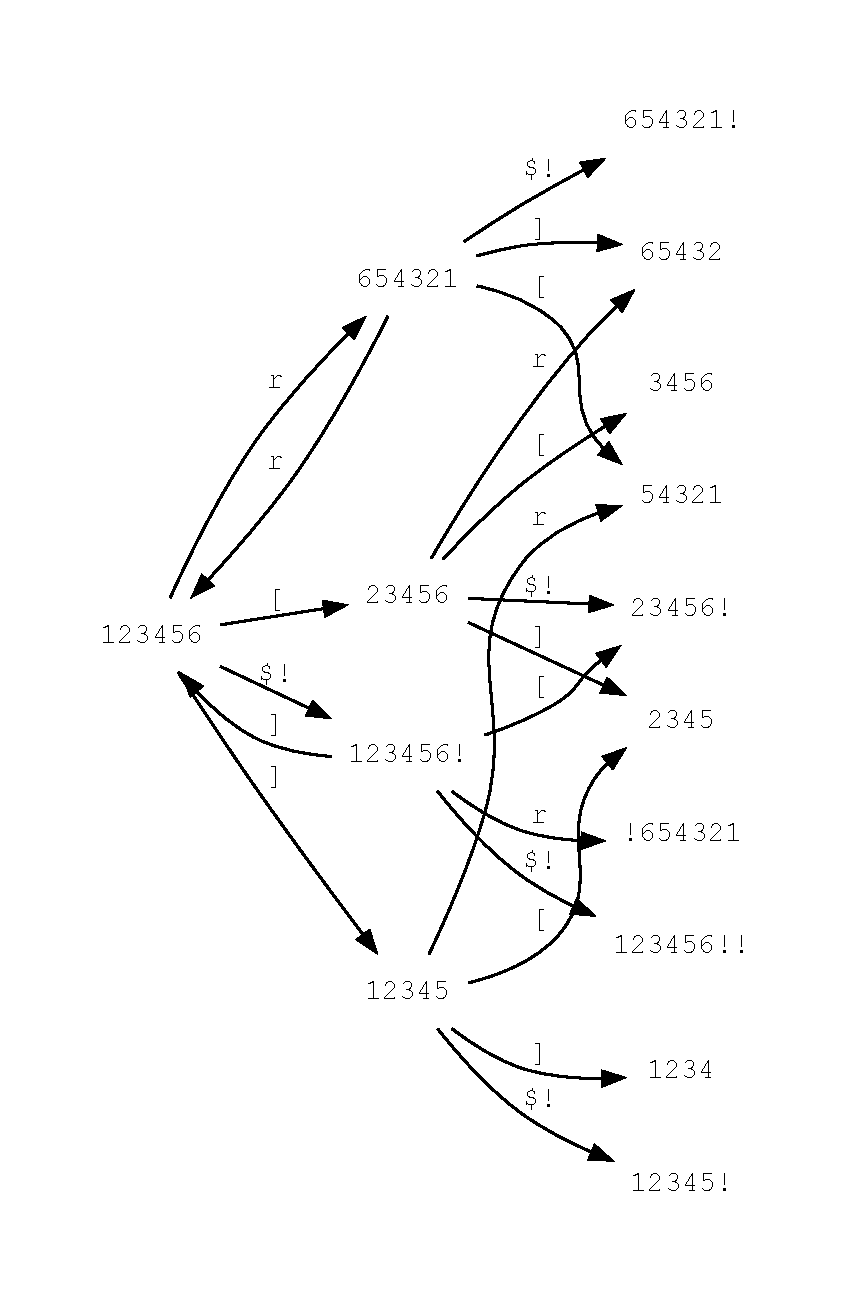
\includegraphics[width=\linewidth]{example-pw-rules.pdf}
\caption{Small example of the combinatorial explosion of passwords generated by
applying primitive rules. Note that some passwords may be reached by several
distinct rule histories, e.g., starting with password `123456,' the password
`54321' may be arrived at by applying complex rules `r [' or `] r,' or
even `\$! r [ [' (not shown in the graph).}
\label{fig:pwgen}
\end{figure}

Figure~\ref{fig:pwgen} shows an example of the combinatorial explosion of
candidates that results from the brute-force algorithm.

\subsection{Optimizations for accuracy}

\subsubsection{Eliminating targets after they are hit}

when a target is hit, do not consider it a target anymore

if we do not do this, algorithm has a tendency to transform complicated
passwords to simple ones by removing characters and adding new ones. but
intuitively, the causal relationship between a simple and complicated password
is the reverse: one expects a simple password to be transformed into a
complicated one by iterative application of rules (e.g., a person first adds a
`1' to the end of their existing password, then later adds a `!' to the front,
etc.)

\subsubsection{Ordering by password strength}

as opposed to arbitrary order

\cite{bonneau2012statistical}

reducing strength for generated but unknown passwords

\subsubsection{Inventing primitive rules}

complex rules that hit enough targets turn into primitives

\subsection{Optimizations for time and memory}

\subsubsection{Use of radix trees}


\subsubsection{Rule simplification}

\begin{table}
\centering
\begin{tabular}{|l|l|l|l|}
\hline
Rule length & Original count & Simplified count & Ratio \\
\hline
1 & 313 & 313 & 1.0 \\
2 & 97,000 & 90538 & 0.93 \\
3 & 30,762,000 & 26,726,754 & 0.87 \\
4 & 296,735,000 & 255,805,952 & 0.86 \\
\hline
\end{tabular}
\caption{Impact of rule simplification. Rule length indicates number of
primitives in each complex rule; e.g., `r ] \$1' has length 3. Original count
specifies the number of rules generated with a certain length, without rule
simplification. Simplified count shows number of rules that remain after
rewriting some to a simpler form. Simpler forms will typically be repeats and
will be removed from the count.}
\end{table}

\subsubsection{No-op rule detection}

detecting a complex rule generates an identical password somewhere in its chain

also check rule positions for rules that use a position arg

\subsubsection{Capping the candidate set}

using the max cycles and chosen set size to limit the number of passwords in
the candidate set

show memory size stat

\section{Experimental Methodology}

choose target set: rockyou, ordered by freq according to pwned hashes (why
ordered by freq)

choose num of cycles

choose candidate group size per cycle

generate passwords

with resulting rule file (which is ordered by rule score), run hashcat on pwned
hashes (most freq 100mil)

compare with: dive, smaller sets of our generated rules, pantagrule, etc.

check num of dups with ours vs others

\section{Results}

our generated rules are intuitively accurate, based on what we think we know
about how people modify their passwords

Table~\ref{tab:top_rules} shows top rules

\begin{table}
\centering
\begin{tabular}{|l|l|l|}
\hline
Rule & Score & Explanation \\
\hline
\$1 & 524,985.0 & Add `1' to end \\
] & 291,809.0 & Remove last character \\
\$2 & 201,185.0 & Add `2' to end \\
T0 & 141,919.0 & Toggle case of first character \\
\$3 & 129,370.0 & Add `3' to end \\
\$7 & 000 & Add `7' to end \\
\$1 \$2 & 000 & Add `12' to end \\
\$4 & 000 & Add `4' to end \\
\$1 \$2 \$3 & 000 & Add `123' to end \\
\$5 & 000 & Add `5' to end \\
\lbrack~\textasciicircum 2 & 000 & Replace first character with `2' \\
r \{ & 000 & Reverse and then rotate left\\
\$2 \$3 & 000 & Add `23' to end \\
\$s & 000 & Add `s' to end \\
\$6 & 000 & Add `6' to end \\
t & 000 & Toggle case of all characters \\
\hline
\end{tabular}
\caption{Top rules generated by our procedure. Scores represent relative
success at matching target passwords (i.e., cracking success).}
\label{tab:top_rules}
\end{table}

memory usage was capped, due to our optimizations

fewer targets were hit over time due to selecting candidates by strength; thus,
also fewer rules were added over time

\begin{figure}
\includegraphics[width=\linewidth]
{../cracked_attempted_plot_23454e5c-a549-11ed-aed9-005056c00001.png}
\end{figure}

\begin{figure}
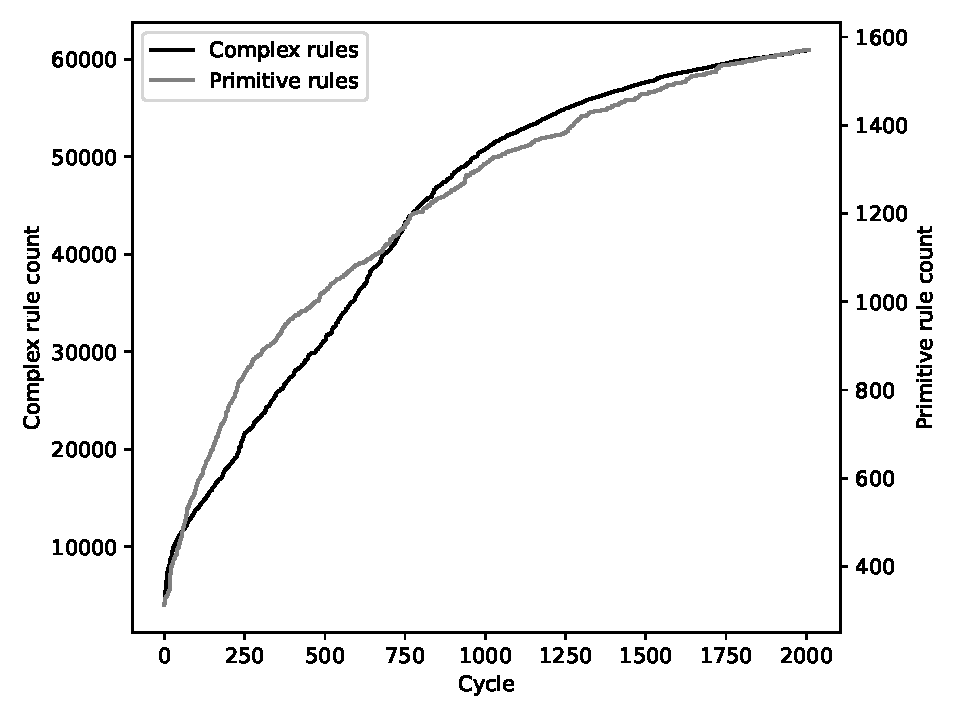
\includegraphics[width=\linewidth]
{analysis/passwords-analysis/stats-rules_composites_size.pdf}
\caption{Growth of complex and primitve rules over time (cycles). As targets
are hit, more complex rules are added. }
\label{fig:rule_count}
\end{figure}

\section{Future Work}

explore use of word dictionaries

boost rule score only if rule produced a stronger password from a weaker one?

\section*{Acknowledgments}

We wish to thank Jonathan Lamoureux for his contributions to this project.

\section*{Availability}

Our code and results are available on GitHub at
\texttt{github.com/joshuaeckroth/passwords}. We used various datasets
to generate our results:

\begin{itemize}
\item RockYou plaintext passwords:
\texttt{github.com/ zacheller/rockyou}
\item Pwned Passwords version 8, ordered by prevalence:
\texttt{haveibeenpwned.com/Passwords}
\item Pantagrule rules: \texttt{github.com/rarecoil/pantagrule}
\end{itemize}

Hashcat was used to measure the performance of rules:
\texttt{github.com/hashcat/hashcat}.
We also used
`duprule,' a duplicate rule detector:
\texttt{github.com/mhasbini/duprule}.


%-------------------------------------------------------------------------------
\bibliographystyle{plain}
\bibliography{\jobname}

%%%%%%%%%%%%%%%%%%%%%%%%%%%%%%%%%%%%%%%%%%%%%%%%%%%%%%%%%%%%%%%%%%%%%%%%%%%%%%%%
\end{document}
%%%%%%%%%%%%%%%%%%%%%%%%%%%%%%%%%%%%%%%%%%%%%%%%%%%%%%%%%%%%%%%%%%%%%%%%%%%%%%%%

%%  LocalWords:  endnotes includegraphics fread ptr nobj noindent
%%  LocalWords:  pdflatex acks
